\section{Simulations and Performance Analysis}
In this section we describe the implementation of our simulator and discuss some performance measurements acquired using this tool. We also describe features that should be added to the simulator to support more realistic experiments. We conclude with a discussion of good parameter selection based on our observations using the simulator.

\subsection{Simulation Design}
To assess the expected overhead introduced by Boomerang we implemented a custom simulator that emulates the behavior of Bitcoin nodes (software clients) running Boomerang. Our simulator has the following properties:
\begin{enumerate}
	\item Nodes enter and exit the network at random times. 
	\item Nodes make new transactions using configuration-specificed parameters $W$ and $D$ at a random rate $\pi$.
	\item Nodes generate cover traffic at a random rate $\sigma$.
	\item Nodes manage their internal address address books according the protocol described in section \ref{sec:design}.
\end{enumerate}

% 1. average time between transaction creation and final broadcast bounded by what?
% 2. average bandwidth consumption by node (based on generation rate)

\subsection{Performance Metrics}
TODO: plots, charts, graphs here

\begin{figure}[ht!]
\begin{center}
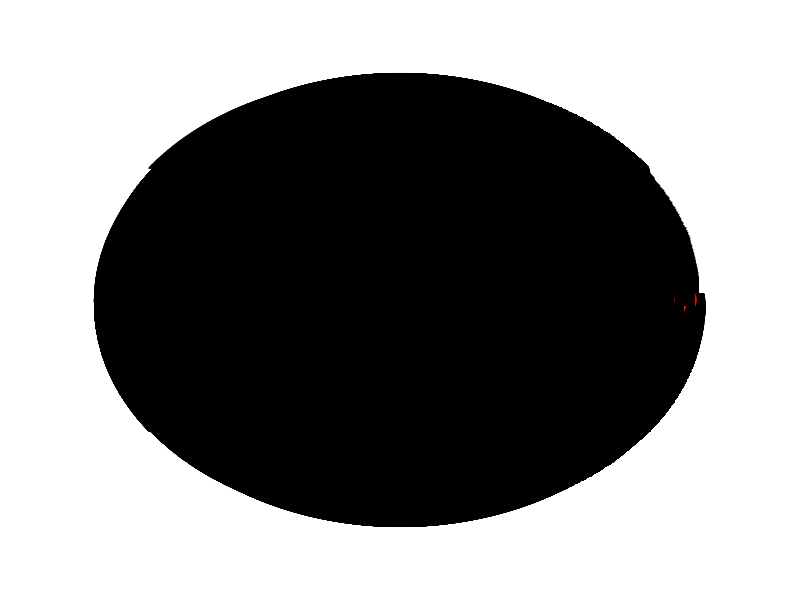
\includegraphics[scale=0.5]{./images/sim_2_complete.png}
\caption{TODO.}
\label{fig:boomerang_message}
\end{center}
\end{figure}

\begin{table*}
\begin{center}
\caption{TODO}
\label{tab:sim-results}
    \begin{tabular}{|l|l|l|l|l|} \hline
    {\bf E[Message Latency]} & {\bf E[Chaff Encryptions]} & {\bf E[Transaction Encryptions]} & {\bf E[Forwarded Messages]} & {\bf E[Retries]} \\ \hline
    ~ & 35.25 & 18.91 & 16468.7 & 0.04 \\
    ~ & 29.59 & 20.75 & 13750.8 & 0.015 \\ \hline
    \end{tabular}
\end{center}
\end{table*}

\subsection{Parameter Selection}

From a performance perspective, our main goal is to minimize the overhead of Boomerang message encoding, transmission, and forwarding while maximizing the anonymity properties discussed in the previous section. To that end, we discuss how the performance varies based on system-wide parameters that influence such anonymity properties. Based on the Boomerang design it is clear that the performance of the Boomerang scheme is tightly coupled to the following paramters:
\begin{itemize}
	\item $W$ - the circuit width,
	\item $D$ - the circuit depth,
	\item $\sigma$ - the average cover traffic generation rate, and
	\item $\pi$ - the average rate at which new transactions are made.
\end{itemize}

Using the custom simulator developed for this project, we propose ****

% cover traffic generation rate (random variable)
% mix buffer delay (random variable)
% circuit length (fixed)
% mix buffer size (fixed)
% encoded transaction size

